\documentclass[conf]{new-aiaa}
%=============================================================
\usepackage[utf8]{inputenc}
\usepackage{graphicx}
\usepackage{amsmath}
\usepackage[version=4]{mhchem}
\usepackage{siunitx}
\usepackage{longtable,tabularx}
\usepackage{fixme}
\DeclareGraphicsExtensions{.ps}
\DeclareGraphicsRule{.ps}{pdf}{.pdf}{`ps2pdf -dEPSCrop -dNOSAFER #1 \noexpand\OutputFile}
\setlength\LTleft{0pt}
\hypersetup{colorlinks=true}
\usepackage{tikz}
\usepackage{subcaption}
\newcommand{\average}[1]{\langle #1 \rangle}
\newcommand{\Rey}{\mathcal{R}\mathfrak{e}}
%=============================================================
\fxsetup{status=draft, layout=inline, theme=color}
%=============================================================
\title{Understanding Dynamic Interaction Between Low Re Aerodynamic Load and Flexible-Biomimetic Wings by FSI Modeling}
%=============================================================
\author{Smail Boughou\footnote{PhD Candidate, smail.boughou@uir.ac.ma , AIAA student member}}
\author{Ashraf A. Omar\footnote{Professor, ashraf.omar@uir.ac.ma, AIAA Senior Member}}
\author{Omer A. Elsayed\footnote{Professor, omer.almatbagi@uir.ac.ma}}
\affil{International University of Rabat (UIR), School of Aerospace and Automotive Engineering, LERMA, Rabat-Sala El Jadida, Morocco}
\author{Radouan Boukharfane
\footnote{Research \& Education Fellow, radouan.boukharfane@um6p.ma, AIAA Member}}
\affil{Mohammed VI Polytechnic University (UM6P), MSDA group, Benguerir, Morocco}
\author{Daniel J. Inman
\footnote{Harm Buning Collegiate Professor of Aerospace, daninman@umich.edu, AIAA Fellow}}
\affil{Department of Aerospace Engineering, University of Michigan, 1320 Beal Ave, Ann Arbor, MI 48109, USA}
%=============================================================
\linespread{1.4}
%=============================================================
\begin{document}
%=============================================================
\maketitle
%=============================================================
\begin{abstract}
Since previous work highlighted the need to evaluate aerodynamic load on airfoil to gain a better understanding of the aero-structural features in turbulent flow conditions.
%
In the present work, we investigate the behavior of flexibility of bio-inspired wings.
%
These wingtips, like avian principle feathers, are meant to control flow.
%
The behavior of the aerodynamic response to the flexible surface of wings are examined.
%
In the course of this work, the validation is performed for a NACA6409 airfoil considering a rigid segment of 40\% and flexible segment 60\% chord length in order to test the aero-structure behavior for an aerodynamic load of air flow at low Reynolds number ($\Rey$) lower tha  $5\times 10^5$.
%
By testing two different Young's modulus ($\mathcal{E}= 689.5$ MPa and $2.5$ GPa), results indicate that the objectives were only partially met for the high $\mathcal{E}$.
%
The results suggest that $\mathcal{E}= 2.5$ GPa is a promising alternative to replicate the feather and will be used in further investigation of the bird-like wings. 
\end{abstract}

\section{Nomenclature}
{\renewcommand\arraystretch{0.8}
\noindent\begin{longtable*}{@{}l @{\quad=\quad} l@{}}
$\mathrm{UAV}$        & Unmanned Aerial Vehicle \\
$\mathcal{U}_\infty$  & Freestream velocity \\
$c$                   & chord length \\
$\nu$                 & kinematic viscosity \\
$\Rey$                & Reynolds Number ($\Rey=\mathcal{U}_\infty c/\nu$) \\
$\mathcal{E}$         & Young's Modulus \\
$\mathcal{L}$         & Flexible Trailing Edge \\
$\Delta t$            & time step \\
$\mathcal{F}_x$       & $X$ component of the resultant pressure force acting on the vehicle \\
$\mathcal{F}_y$       & $Y$ component of the resultant pressure force acting on the vehicle \\
$t^*$                 & time period \\
\end{longtable*}}
%=============================================================
\section{Introduction}
%=============================================================
\lettrine{T}he comparison of the aerodynamic efficiency of gliding birds against UAVs is insightful for a better understanding of natural flight.
%
There has been an increased recognition that more attention needs to be paid to morphing wings. Wing morphing allows gulls to modulate static pitch stability during gliding \cite{harvey2022birds}. 
%
The morphing ability of the flexible membrane wing is provided by its flexibility, which allows it to adaptively alter the shape under aerodynamic loading.
%
The aerodynamic performance modeling and flow control are drawing the interest of zoologists, biologists, and the concerned aerodynamics community.
%
As a result, these researches combine the biological theory of natural flying with aerodynamic methodologies to address MAVs based on bird endurance.
%
Flexible wing is a successful way for improving the aerodynamic robustness of tiny fixed wing drones operating in uncertain air situations by using a revolutionary biomimetic design.
%
The aim is to introduce a multidisciplinary approach to the study of biologically influenced flights by coupling aerodynamics, structure, and flight mechanics.
%

The birds wing aerodynamic is different in behavior compared to the conventional man-made wings as \citet{withers1981aerodynamic} found that the bird wings perform with low drag generally had low maximum lift coefficients, whereas wings with high maximum lift coefficients had high drag coefficients. 
%
Their wings are models for the construction as noise reducing application \cite{bachmann2010anatomical}.
%
Early studies on experimental biology focused on the material properties testing of the biological flights such as the wings and feathers structures \cite{bachmann2012flexural}.
%
Among the studied species is the owl. They are known for their silent flight because of the features in its wings that promote smooth flow \cite{jaworski2020aeroacoustics,geyer2016silent}.
% 
Implementation of biomimetic approach is meant to replicate the feather effects on aerodynamic performance \cite{hedenstrom2017wind}. 
%
A thin and feather-like shapes that have a finite trailing edge thickness were designed by \citet{ananda2018aerodynamic} by using a multi-point inverse airfoil design technique in PROFOIL \cite{AirfoilDesignSoftwarefortheWeb} to design airfoil families (AS6091 to AS6099).
%
It consists of modifications in the finite trailing thickness between 4\%–6\% and can perform efficiently at the same bird Reynolds number scales ($10^4$-$10^5$).
%
\citet{harvey2022review} focused their survey on various possible controls provided by bio-inspired morphing that engineering studies could validate and incorporate to enhance flight maneuverability.
%
Using morphing mechanisms including camber morphing techniques, wing morphing can be utilized to alter lift distributions and generate longitudinal control (cf. Fig.~\ref{fig:camberMorphing}.
%
\begin{figure}[ht!]
\centering
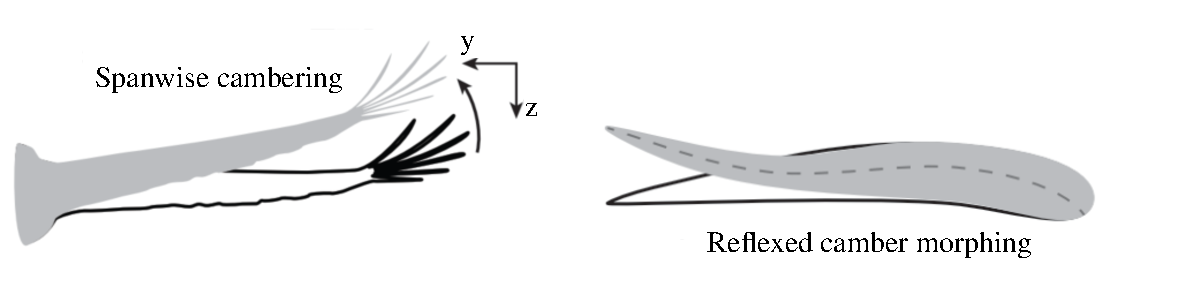
\includegraphics[width=0.9\textwidth]{figs/morph-crop.pdf}
\caption{Different UAV implementations of avian-inspired wing camber morphing spanwise cambering and chord-wise morphing \cite{harvey2022review}.}
\label{fig:camberMorphing} 
\end{figure}
%
A deeper understanding of their control response in dynamic and turbulent environments is required, concluded the review.
%
This camber-morphing airfoil method extends prior work by its unique consideration of the instantaneous flow control \cite{gamble2020aeroelastic,gamble2020load}.

Although some attempts have been made to address morphing wings, much of the work in this area is limited to steady CFD predictions of the original and morphing airfoils.
%
As a first step to understanding how the flow responds to dynamic morphing flap deflection,  insightful work is presented by \cite{abdessemed2018morphing} using dynamic meshing to perform CFD analyses.
%
The NACA 0012 airfoil fitted with a morphing trailing edge (TE) flap showed potential for future applications. 
%
Here it is reported that those studies neglected the dynamic aspect of the interaction between fluid and wings.
%
In these directions, a growing field of researchers studying and developing avian-inspired morphing aircraft focused on the study of the morphing wings.
%
\citet{gamble2020aeroelastic} found that the bio--inspired flexible airfoil maintained lift at Reynolds numbers below $1.5\times 10^5$, but at greater Reynolds numbers, the flexible airfoil alleviated the lift force and experienced trailing edge displacement.
%
\citet{murayama2021flexible} in their study showed the effectiveness of flexible flaps inspired by bird feathers can improve aerodynamic robustness in low Reynolds number wings.
%
It reduces the fluctuations of aerodynamic forces in a perturbed flow behind an oscillating plate by suppressing large-scale vortex shedding. 
%
In previous work on understanding the low Re aerodynamic phenomena encountered while studying the owl-like airfoil \cite{boughou2022low} showed the unsteadiness of the aerodynamic coefficients.
%
The aero-structural response to the aerodynamic load is the motive behind the work presented in this paper.

The role of feather morphing hasn't been thoroughly investigated, and its impact on aerodynamics is unknown. 
%
The aero-structural response of a flexible airfoil designed using biologically inspired structural and material data from feathers requires studies that concentrate on evaluating aerodynamic load and the aero-structural features in turbulent situations.
%
In the current study on bio-inspired flexible wings, we aim to make use of existing research in the field and complete several objectives. 
%
First, we examine bio-inspired structure requirements  necessary to capture both flow field and structural analysis. 
%
Computational modeling can provide a way to develop predictive relationships between morphological traits and their impact on aerodynamic performance through a series of flexibility conditions that will be computed using Fluid-Structure interaction (FSI).
%
One of the primary objectives of evaluations is to investigate the dynamic interaction between Low Re aerodynamic flow and Flexible-Biomimetic NACA6409 as earlier recommended in Ref \cite{gamble2020load} at an angle of attack $15^{\circ}$.
% 
Furthermore, the secondary goal of the study is to investigate and assess feather-like airfoils that resemble a cross-section of a bird wing \cite{murayama2021flexible}, which are narrow plate-like feathers that expand toward the trailing edge. 
%=============================================================
\section{Methods and Material}
%=============================================================
To resolve well-known computational aerodynamics and aeroelastic airfoils, an FSI solver is combined with the turbulence model k-$\omega$ SST and large deformation updated Lagrangian finite volume structure solver \cite{cardiff2014large}.
%
%
\begin{figure}[ht!]
\centering
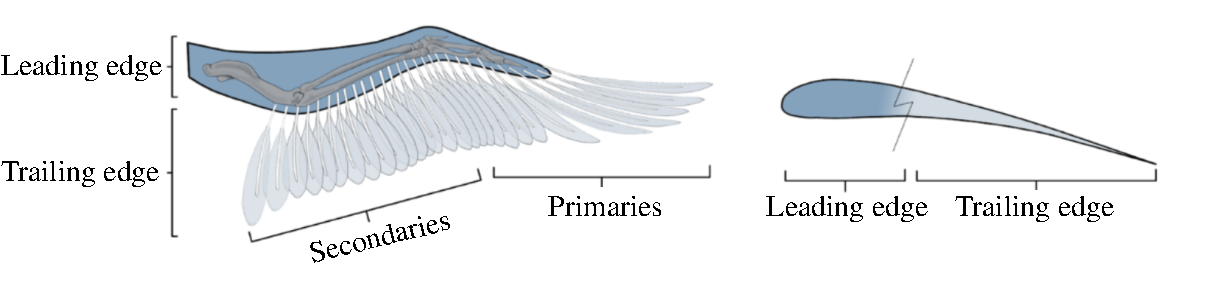
\includegraphics[width=0.9\textwidth]{figs/gamble-crop.pdf}
\caption{Anatomy of bird airfoil considering rigid and flexible segments \cite{gamble2020aeroelastic}.}
\label{fig:segments}
\end{figure}
%
As a first step for the ongoing numerical simulations, the validations based on NACA6409 are performed and compared to the results of previous experiments \cite{gamble2020aeroelastic}.
%
The previous work of \citet{gamble2020load} considered the modelling of feather-like airfoil as two part segments: rigid part and flexible one (cf. Fig.~\ref{fig:segments}).
The rachis' structure mimics that of a narrow cavity in general, with a circular cross section at the root and a rectangular cross section at the trailing edge.
%
\citet{bachmann2012flexural} provided in various biological experiments on the rachis, different material properties such as the Young's modulus $\mathcal{E}$ (Modulus of elasticity).
%
Following the work of \cite{gamble2020aeroelastic}, we use simplified bird airfoil as the basis for this computational study and a Young's modulus $\mathcal{E}$ of both 2.5 GPa and  689.5 MPa chordwise stiffness that may allow feather replication with a constant Young's modulus, through \cite{gamble2020load} used a $\mathcal{E}$ variable ranging [$2.5$-$0.5$ GPa] in stiffness characteristics towards the tip of the feather’s trailing edge.

Airfoil configuration and computational mesh used for the fluid–solid interaction problem is displayed in Fig.~\ref{fig:Ggeometry}.
%
As shown in Fig.~\ref{fig:Griddomain}, the computational domain is built with a structured grid using the ANSYS multi-blocks grid ICEM tool, with the appropriate boundary conditions.
%
The mesh plane is extruded in span wise direction with a one cell.
%
FSI Simulations are performed with an open-source finite volume toolbox for solid mechanics and fluid-solid interaction simulations.
%
The finite volume method described in \citet{cardiff2018open} for orthotropic bodies subjected to large strains and large deformations with consideration of updated Lagrangian finite volume solver \cite{tukovic2014openfoam} is implemented in the FSI method described in this work.
%
The next section \ref{sec:preliminary} outlines the preliminary resulting data assessed in multiple stages of the study of the NACA6409 airfoil (cf. Fig.~\ref{fig:6409}) at Reynolds number of $10^5$ to $5\times 10^5$ considering a rigid segment of 40\% and flexible segment 60\% chord length (cf. Fig.~\ref{fig:airfoilSegments}).
%
\begin{figure}[ht!]
\centering
\begin{subfigure}{.4\textwidth}
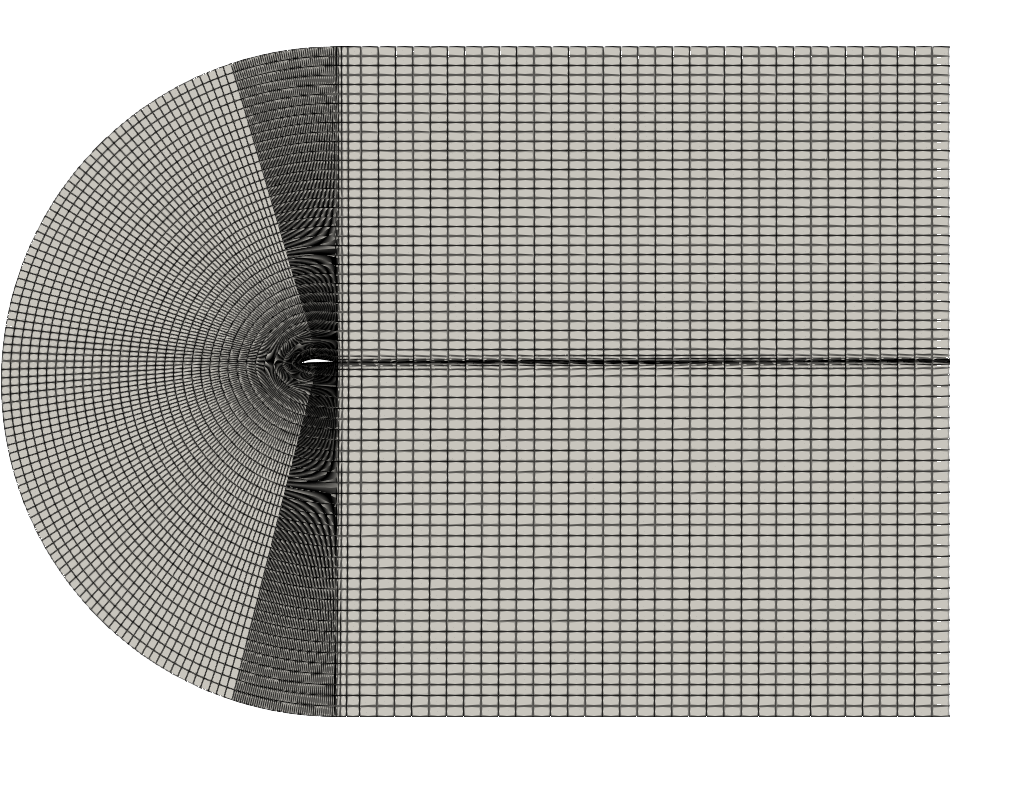
\includegraphics[width=2.8in]{Figures/mesh fluid.png}
\caption{\label{fig:Griddomain} Grid domain}
\label{fig:airfoildesigna}
\end{subfigure}
\begin{subfigure}{.4\textwidth}
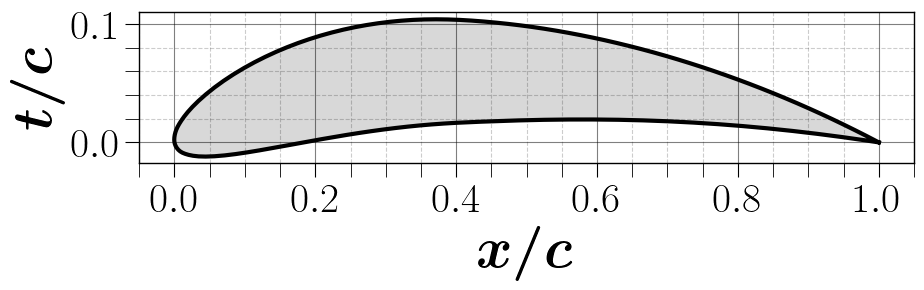
\includegraphics[width=.6\columnwidth]{Figures/naca_airfoil.png}
\caption{\label{fig:6409}NACA6409}
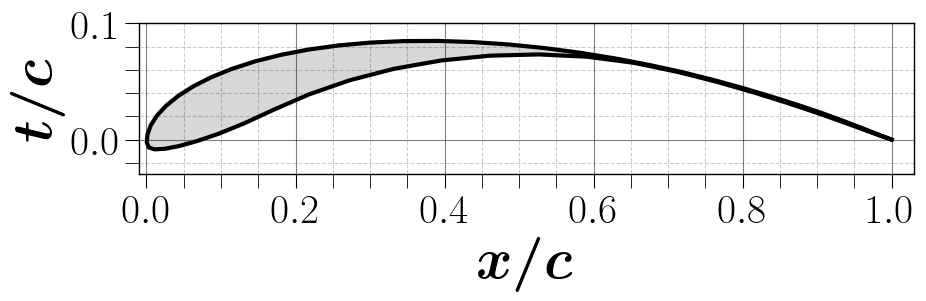
\includegraphics[width=.6\columnwidth]{Figures/AS9065_airfoil.png}
\caption{\label{fig:AS6095}AS6095 airfoil \cite{ananda2018design}}
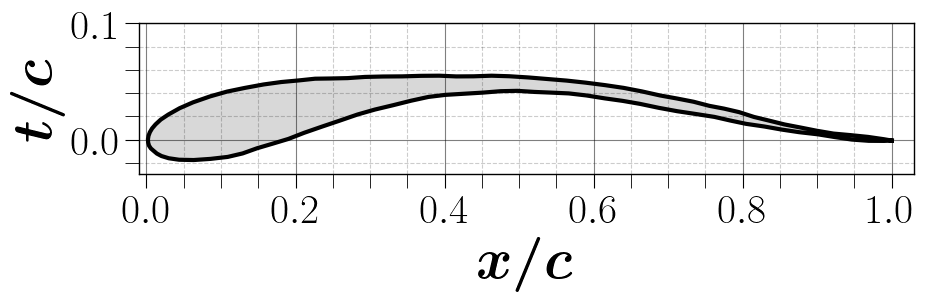
\includegraphics[width=.6\columnwidth]{Figures/owl_airfoil.png}
\caption{\label{fig:owl}Owl airfoil \cite{liu2004avian}}
\end{subfigure}
\caption{Computational domain and airfoil profiles.}
\label{fig:Ggeometry}
\end{figure}
%
In addition, it identifies avenues for further assessment of the man-made-bird-like AS6095 airfoil (cf. Fig.~\ref{fig:AS6095}) designed by \citet{ananda2018design} at a moderate low Reynolds number of $10^5$. Further,  a case study investigates the flow behavior for the known owl-like airfoil (cf. Fig.~\ref{fig:owl}) operating at very low Reynolds of $2.3\times 10^4$.
%
\begin{figure}[ht!]
\centering
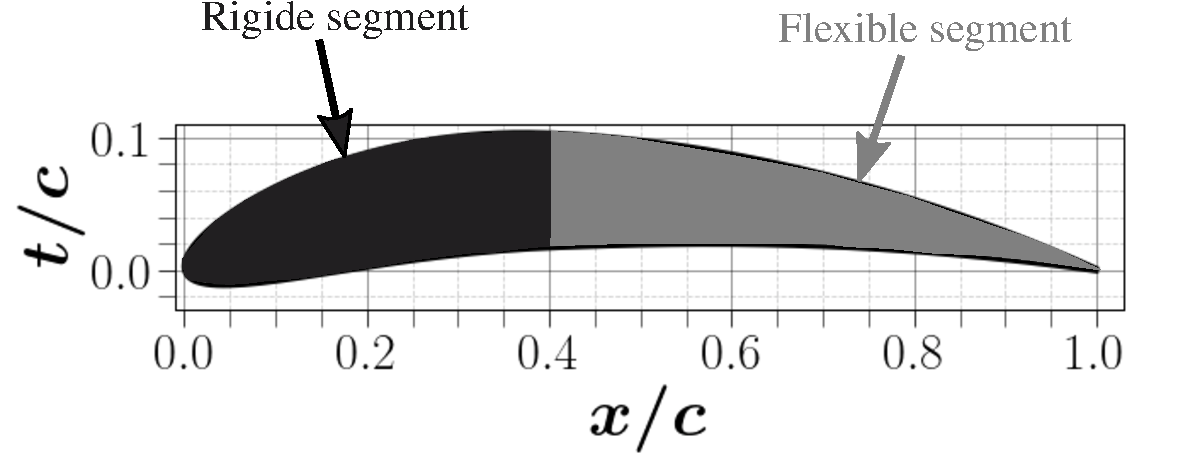
\includegraphics[width=0.70\textwidth]{figs/airfoilgeo-crop.pdf}
\caption{NACA6409 airfoil segments (40\% ) rigid and (60\%) flexible denoted $\mathcal{L}$}
\label{fig:airfoilSegments} 
\end{figure}
%=============================================================
\section{Preliminary Results}
\label{sec:preliminary}
%=============================================================
As a preliminary assessment, a constant Young's modulus can indeed be used with reasonable thicknesses along the chord.
%
The purpose is to provide a strict verification benchmark and this test case serves more for demonstration purposes.
%
An investigation of the Fluid and structure response to different Reynolds number and Young Modulus $\mathcal{E}$ is discussed in the following sections, and each aspect of the FSI will be presented in relation to the findings  at a fixed moderate angle of attack of $15^{\circ}$.
%
Differences in the tip deflection (cf. Sec. \S\ref{sec:deflection}) and fluid-structure response are described in the following sections (cf. Sec. \S\ref{sec:fluidStrucutreRespnseToYoungAndRey}).
%=============================================================
\subsection{Tip deflection}
\label{sec:deflection}
%=============================================================
Here some results of the FSI implementation are illustrated for both Young's modulus 689.5 MPa and 2.5GPa and shown in Figure \ref{fig:history}.
%
The tip deflection history is shown in function of the displacements in the longitudinal direction for the tip control point on the trailing edge.
%
It illustrates the numerical computation of FSI which is performed in two stages.
%
The standard approach for coupling fluid and structural solvers is to solve the fluid dynamic equations first, then transfer the computed loads to the structural equations.
%
First the transient fluid flow is computed without coupling the fluid and structure interaction considering the whole airfoil as rigid body.
%
After the flow is developed along the wing, the system is coupled at a coupling time period of t$^*=0.9$ s and takes into account the flexible segment of the airfoil.
%
An initial comparison between used Young's modulus $\mathcal{E}=2.5$ GPa in literature and  a reduced one E = 689.5 MPa can be done using the preliminary results obtained for $\Rey10^5$ case.
%
In terms of the amount of deflection, the case with $\mathcal{E}=689.5$ MPa shows a maximum value of deflection $10\%$ of the flexible part (we denote $\mathcal{L}$) (cf. Fig.~\ref{fig:deflection689.5MPa}).
%
\begin{figure}[ht!]
\centering
\begin{subfigure}{.45\textwidth}
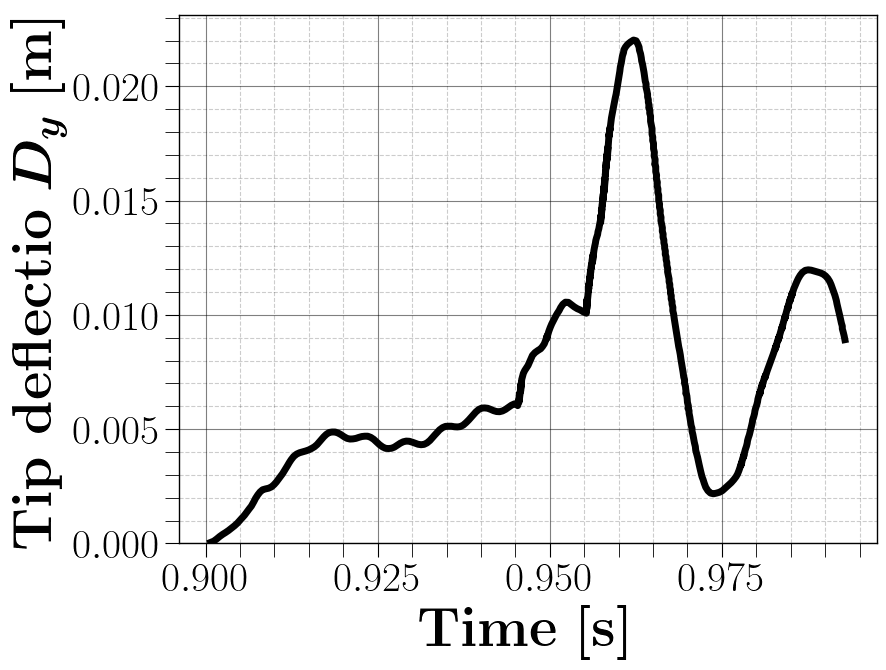
\includegraphics[width=0.99\columnwidth]{figs/deflection689MPa090.png}
\caption{$\mathcal{E}=689.5$ MPa}
\label{fig:deflection689.5MPa}
\end{subfigure}
\begin{subfigure}{.45\textwidth}
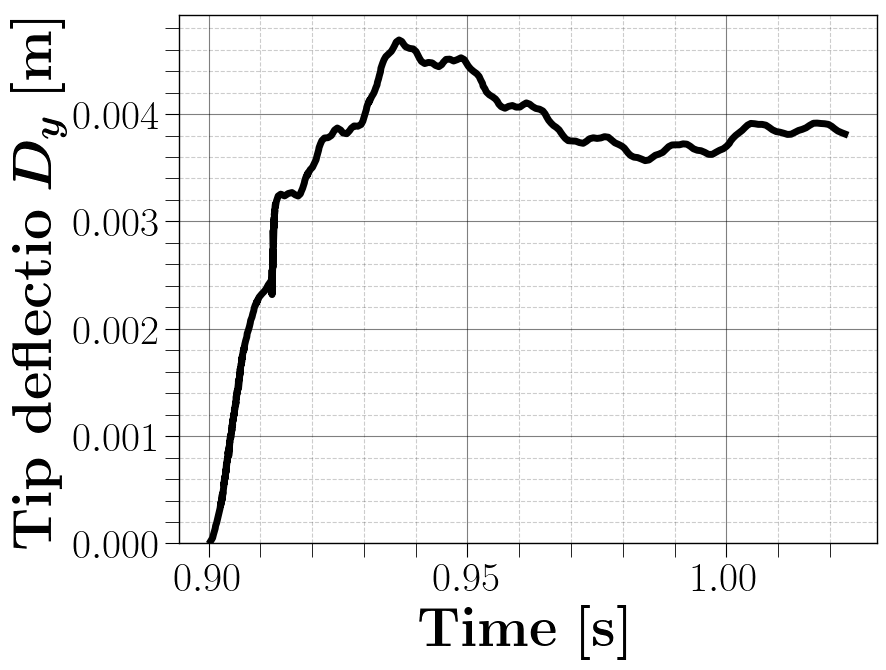
\includegraphics[width=0.99\columnwidth]{figs/deflection25GPa10.png}
\caption{$\mathcal{E}=2.5$ GPa}
\label{fig:deflection2.5GPa}
\end{subfigure}
\caption{\label{fig:history} Tip deflection in y direction at $\Rey =10^5$; (a) Young modulus $\mathcal{E}=689.5$ MPa  (b) $\mathcal{E}=2.5$ GPa }
\label{fig:history}
\end{figure}
%
However, the tip deflection is thought to remain in fluctuation motion.
%
Unlike the previous deformation, and for a Young's modulus $\mathcal{E}=2.5$ GPa, this displacement of the trailing edge tip is deflecting upwards in the same direction of the freestream velocity $\mathcal{U}_\infty$ with a maximum value of deflection $2.2\%$ of $\mathcal{L}$ (cf. Fig.~\ref{fig:deflection2.5GPa}).
%
The results from $\mathcal{E}=2.5$ GPa show a limited amount of fluctuations and demonstrate a state of slowdown. 

%=============================================================
\subsection{Fluid-structure response}
\label{sec:fluidStrucutreRespnseToYoungAndRey}
%=============================================================
To assess the displacement in the longitudinal direction, the modal shapes of structural displacement fluctuations for Young modulus $\mathcal{E}=689.5$ MPa  and $\mathcal{E}=2.5$ GPa, respectively, is displayed in Fig.~\ref{fig:dispMagni}.
%
\begin{figure}[ht!]
\centering
\begin{subfigure}{.45\textwidth}
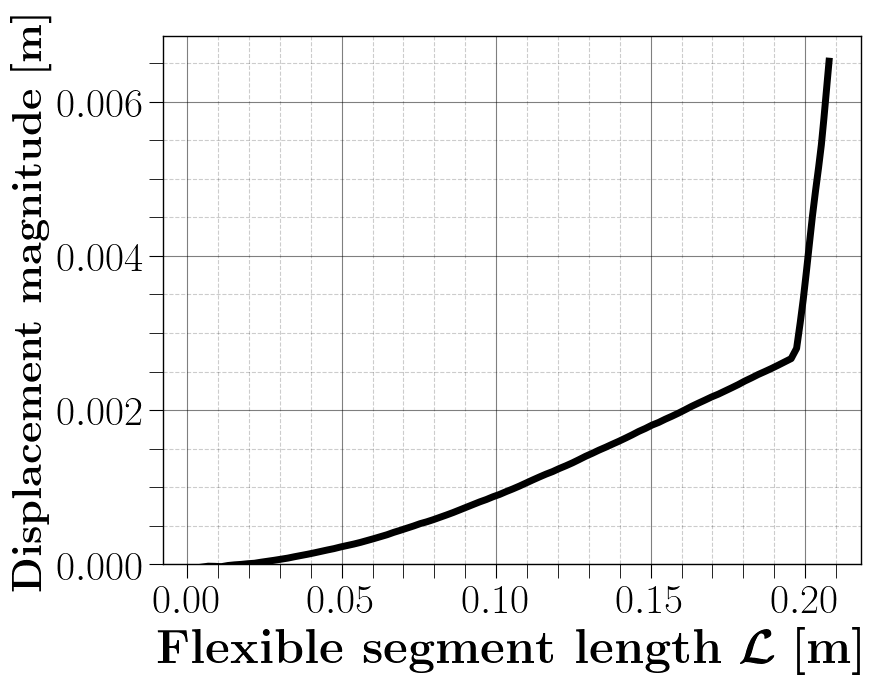
\includegraphics[width=0.99\columnwidth]{figs/dispmagnitude689MPa.png}
\caption{$\mathcal{E}=689.5$ MPa}
\label{fig:dispMagni689.5MPa}
\end{subfigure}
\begin{subfigure}{.45\textwidth}
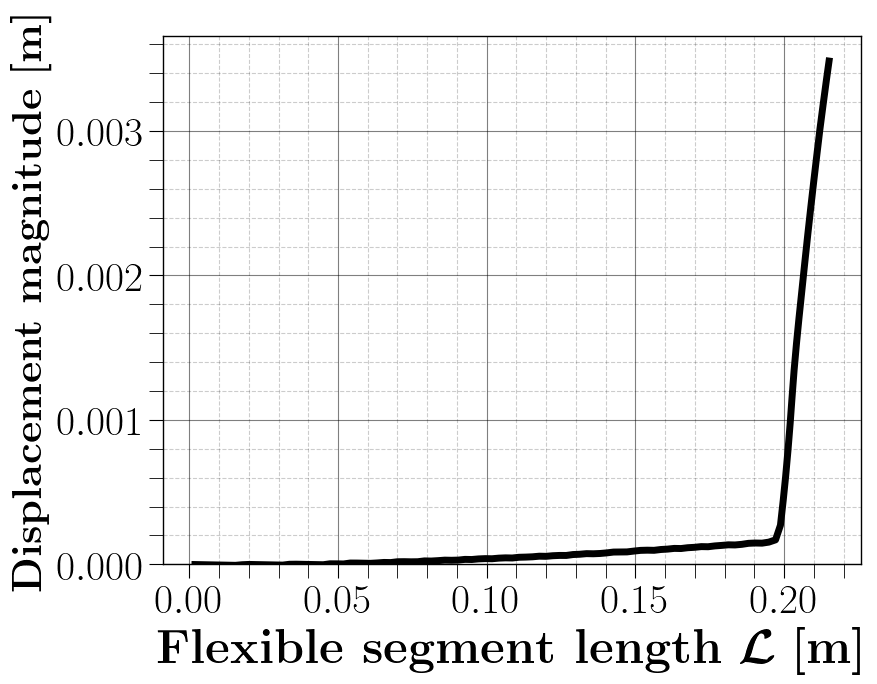
\includegraphics[width=0.99\columnwidth]{figs/dispmagnitude25GPa.png}
\caption{$\mathcal{E}$ = 2.5GPa}
\label{fig:deflection2.5GPa}
\end{subfigure}
\caption{Displacement magnitude distribution at (a) Young modulus $\mathcal{E}=689.5$ MPa (b) $\mathcal{E}= 2.5$ GPa}
\label{fig:dispMagni} 
\end{figure}
%
The distribution of the displacement over the flexible segment $\mathcal{L}$ grow bigger towards the wing tip owing to large displacements at the tip for both values of $\mathcal{E}$.
%
Though, the lower $\mathcal{E}$ exhibits higher tip deflection.
%
Despite the differences, these displacement distribution provide support that the high $\mathcal{E}$ generates a suddenly increase in deflection.
%
\begin{figure}[hbt!]
\centering
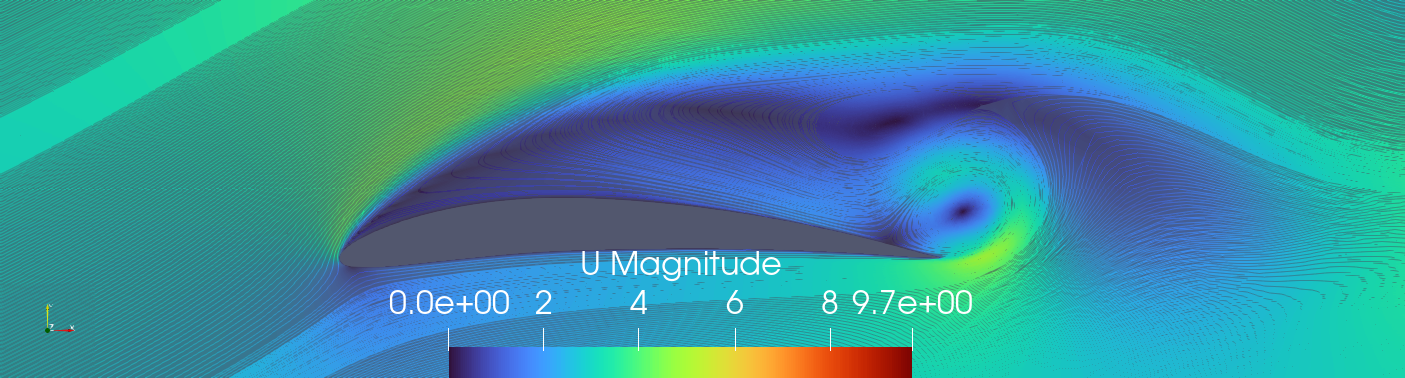
\includegraphics[width=0.45\columnwidth]{Figures/streamLines0906Coupling.png}
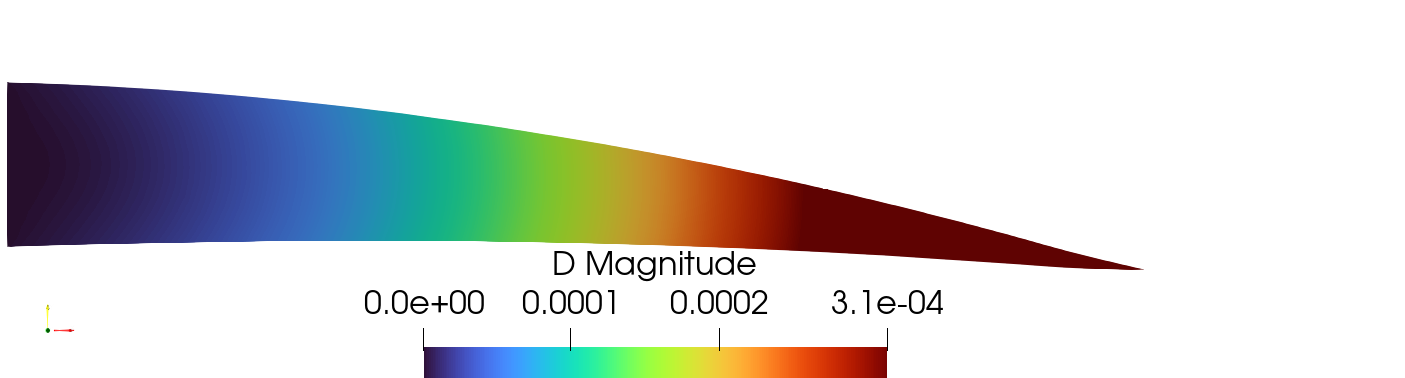
\includegraphics[width=0.45\columnwidth]{Figures/DMAgnitude0906Coupling.png}
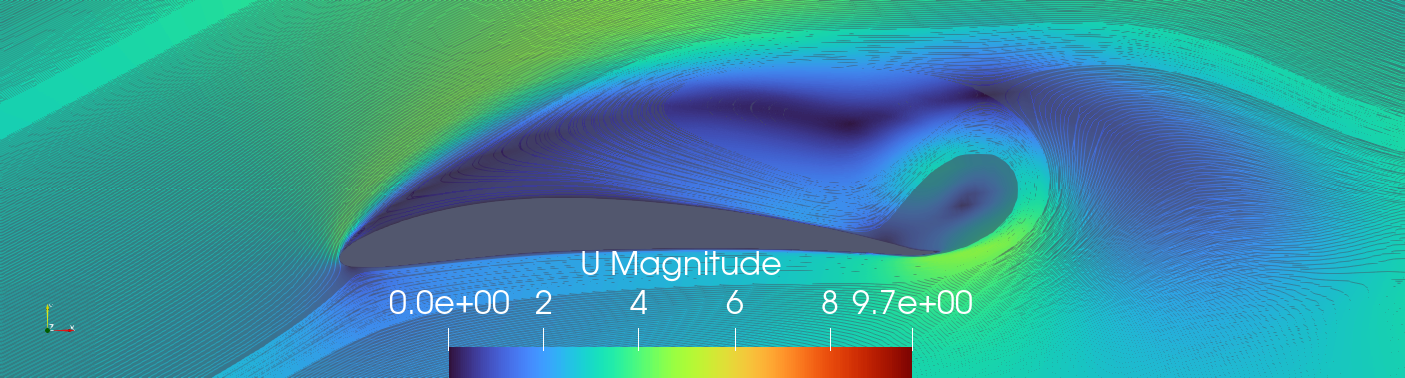
\includegraphics[width=0.45\columnwidth]{Figures/streamLines0918Coupling.png}
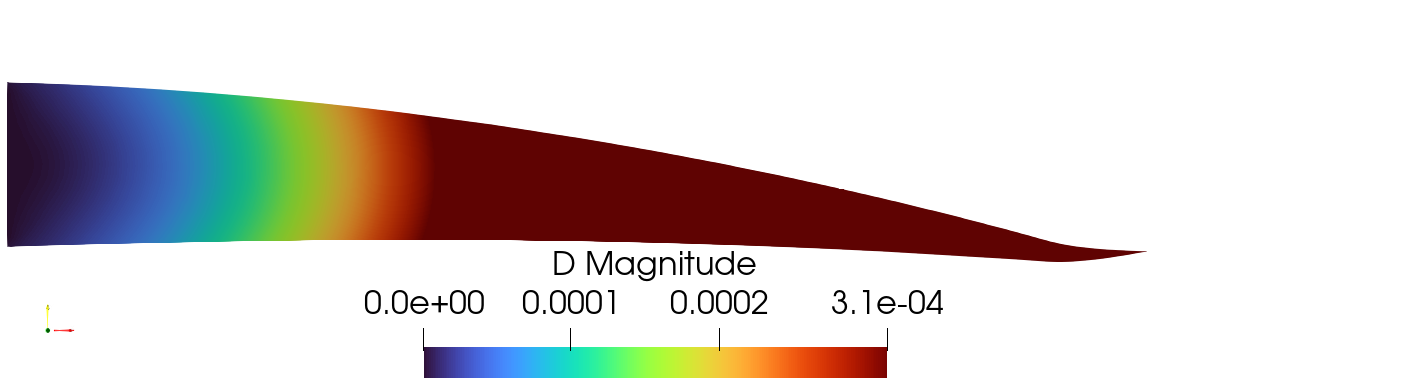
\includegraphics[width=0.45\columnwidth]{Figures/DMAgnitude0918Coupling.png}
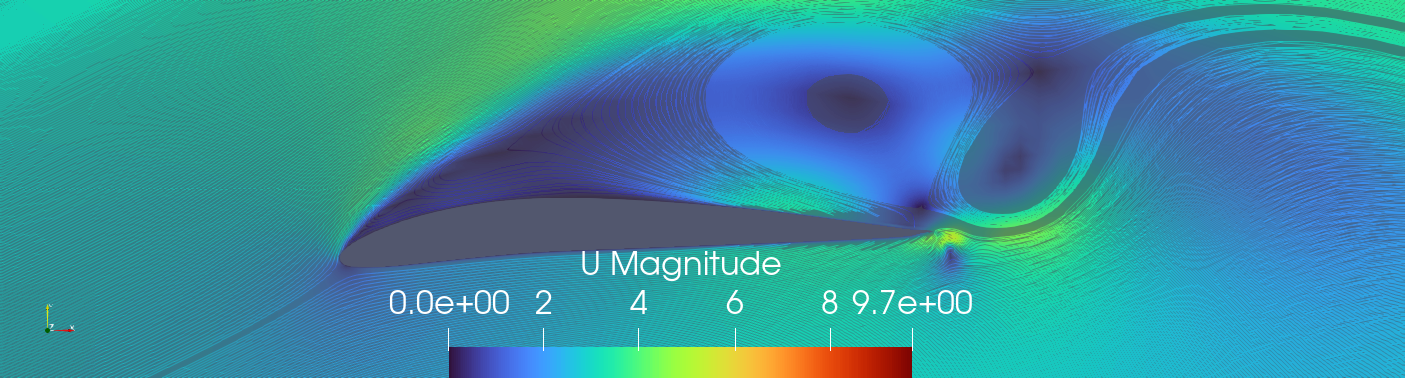
\includegraphics[width=0.45\columnwidth]{Figures/streamLines0958Coupling.png}
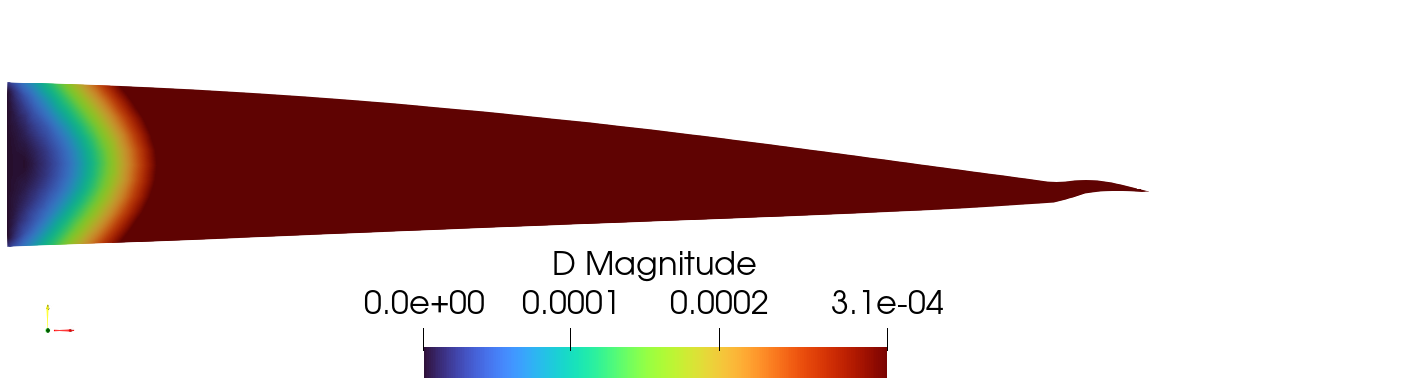
\includegraphics[width=0.45\columnwidth]{Figures/DMAgnitude0958Coupling.png}
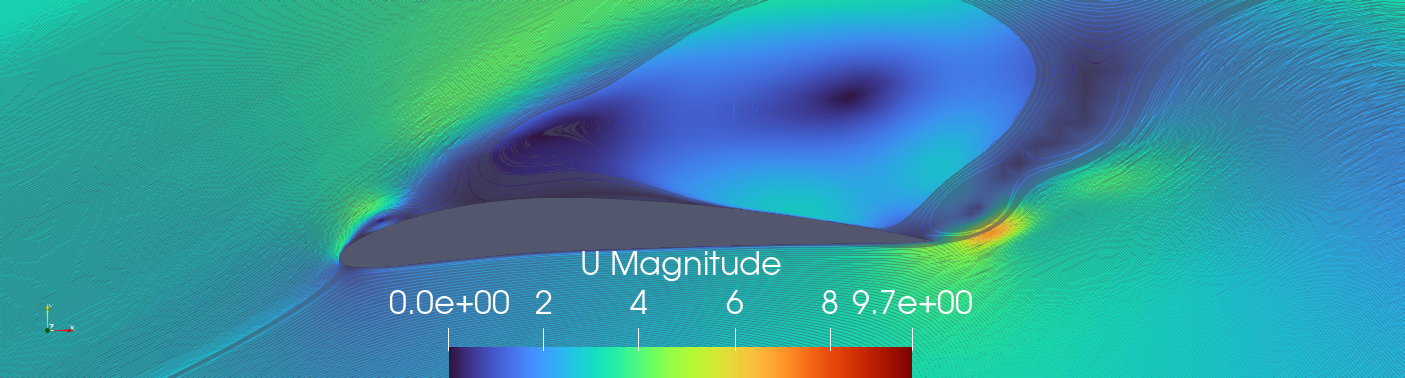
\includegraphics[width=0.45\columnwidth]{Figures/streamLines0986Coupling.png}
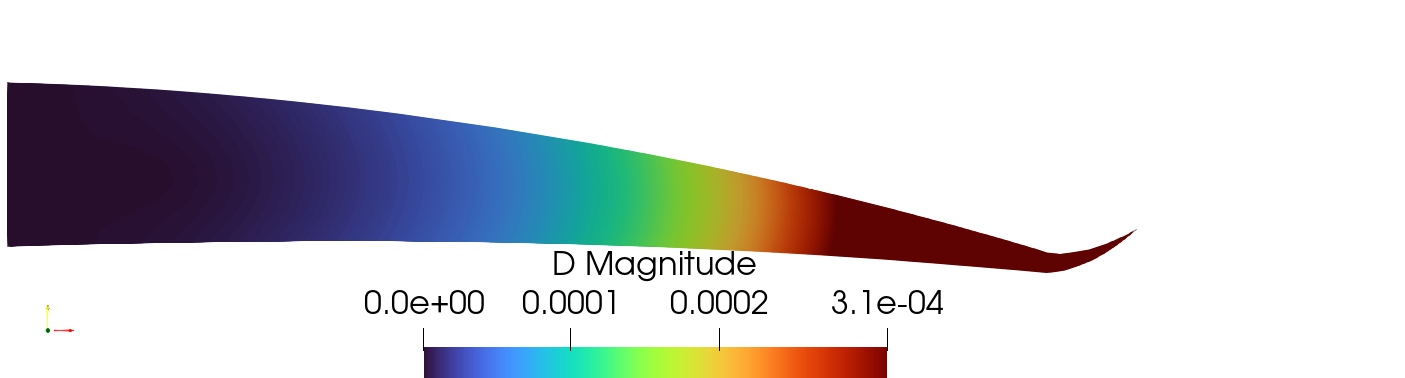
\includegraphics[width=0.45\columnwidth]{Figures/DMAgnitude0986Coupling.png}
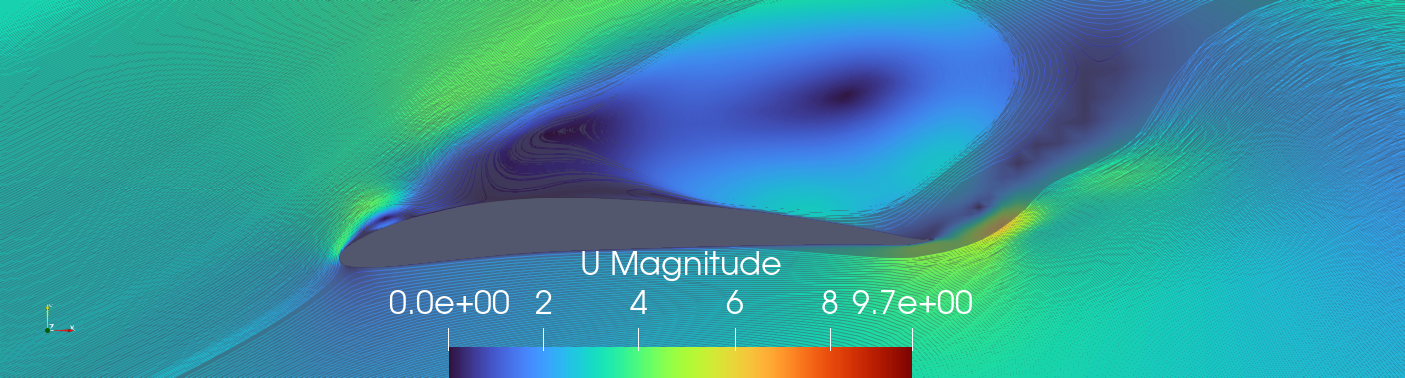
\includegraphics[width=0.45\columnwidth]{Figures/streamLines0988Coupling.png}
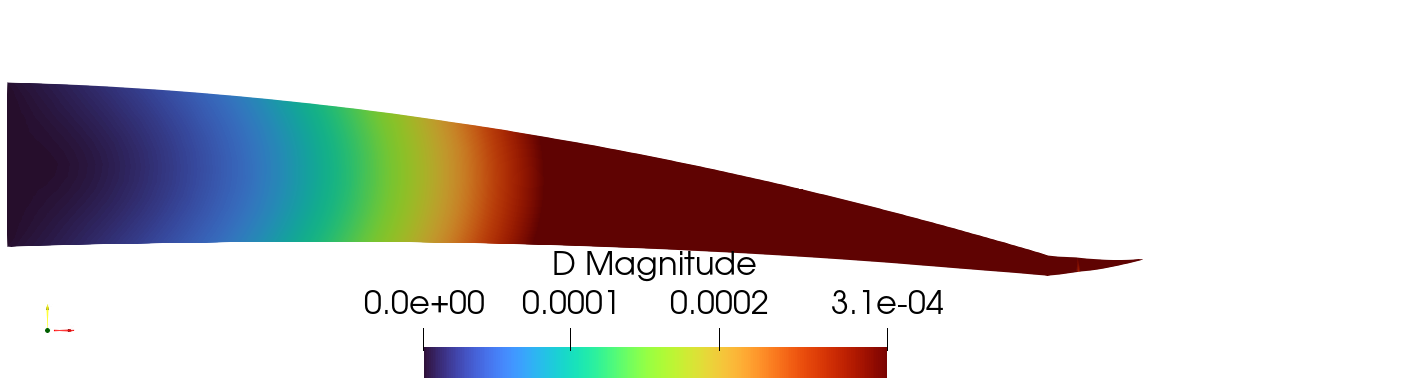
\includegraphics[width=0.45\columnwidth]{Figures/DMAgnitude0988Coupling.png}
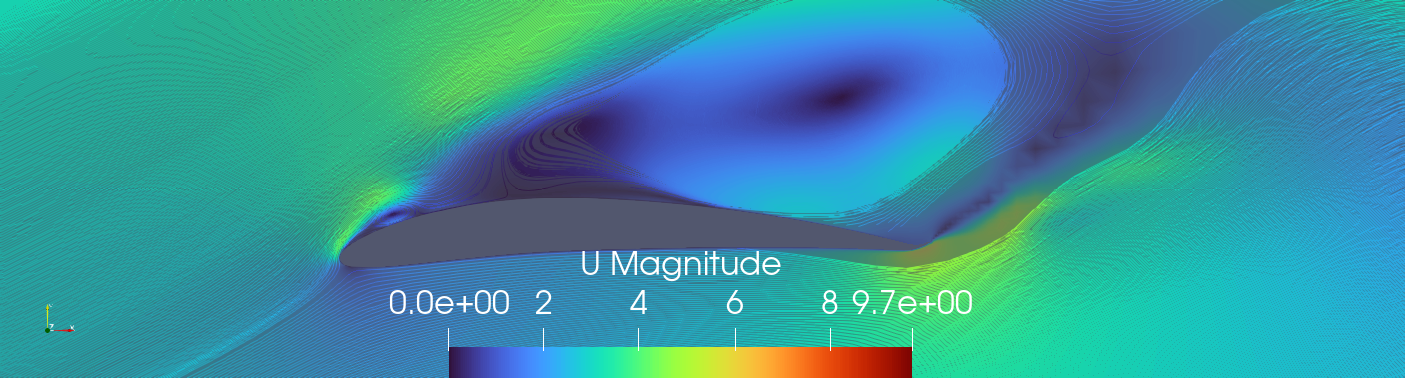
\includegraphics[width=0.45\columnwidth]{Figures/streamLines0992Coupling.png}
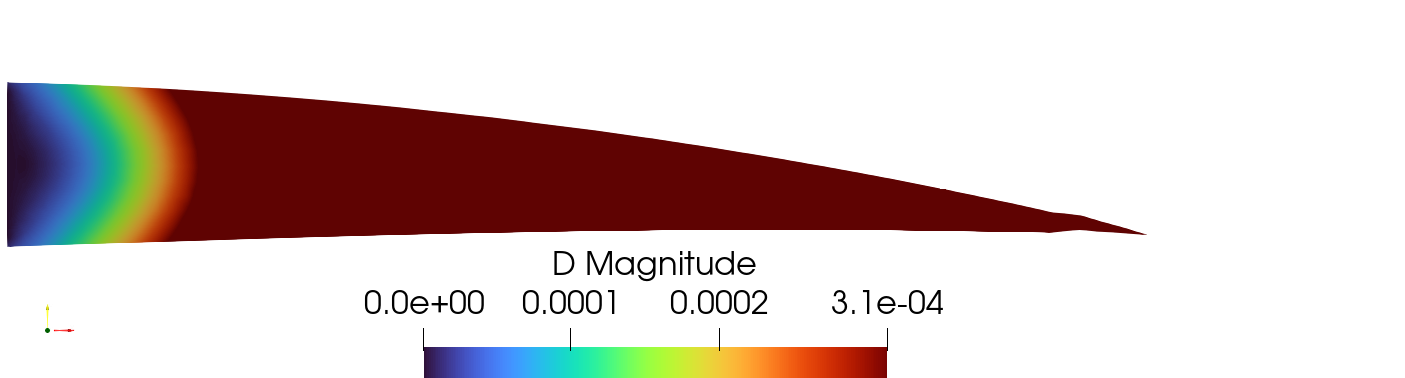
\includegraphics[width=0.45\columnwidth]{Figures/DMAgnitude0992Coupling.png}
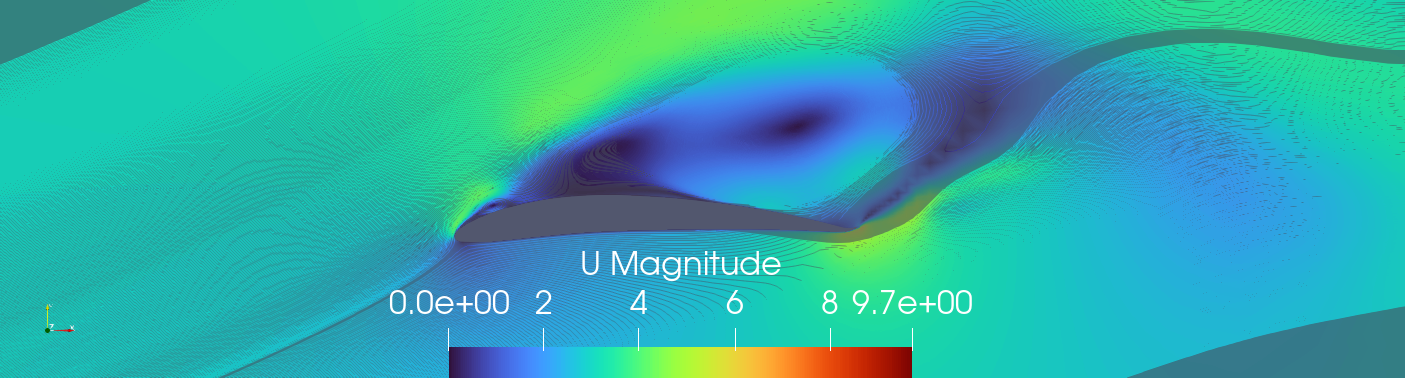
\includegraphics[width=0.45\columnwidth]{Figures/streamLines0998Coupling.png}
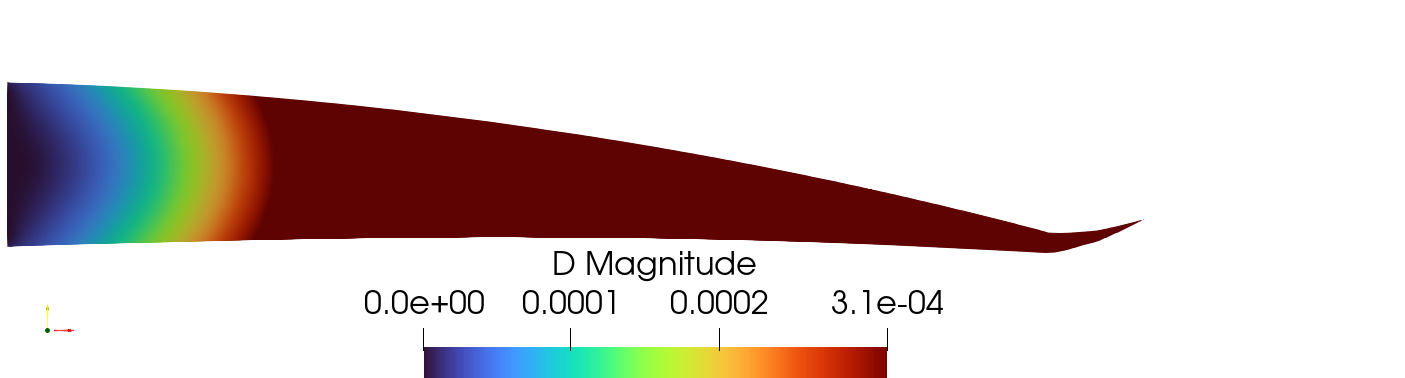
\includegraphics[width=0.45\columnwidth]{Figures/DMAgnitude0998Coupling.png}
\caption{Velocity colored flowfield streamlines (right) displacement contours (left) $\Rey=10^5$ and $\mathcal{E}=689.5$ MPa}
\label{fig:velocityDisplacement} 
\end{figure}
%
The computed instantaneous velocity colored streamlines are shown in Fig.~\ref{fig:velocityDisplacement} (left figures) for $\mathcal{E}= 689.5$ MPa  as well as the corresponding displacement magnitude contour of the flexible segment (right figures).
%
A small trailing edge bubble is formed and increases in diameter.
%
These separation bubbles come in a variety of sizes depending on the tip deflection.
%
For $\mathcal{E}=2.5$ GPa, it is not unexpected to see a small fluctuation of the tip and tends to be stable with the fluid flow over the flexible segment. Therefore the stable state of the tip deflection is highlighted in Fig.~\ref{fig:25GPA} and shows it relaxes towards steady-state structure.
%
%
\begin{figure}[ht!]
\centering
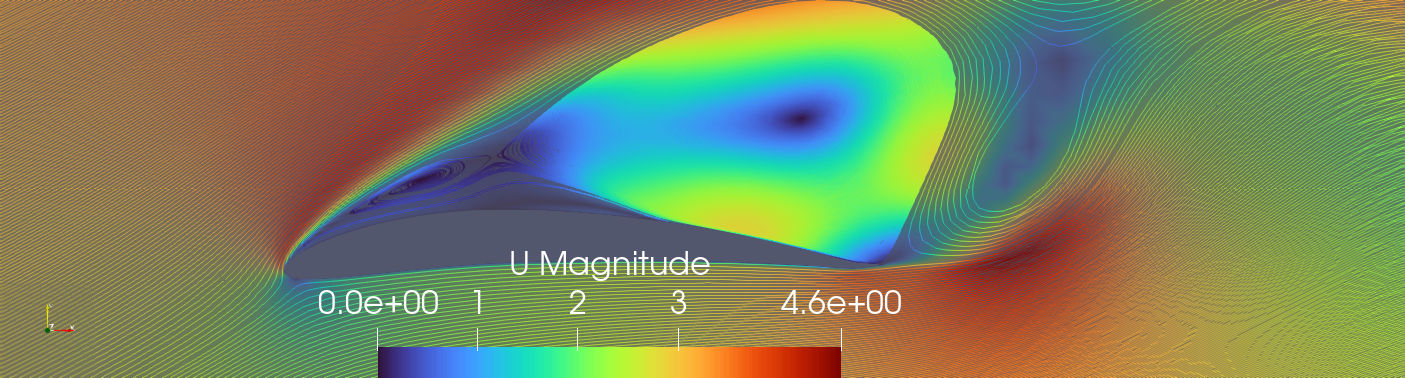
\includegraphics[width=0.45\columnwidth]{Figures/streamLines25GPACoupling.png}
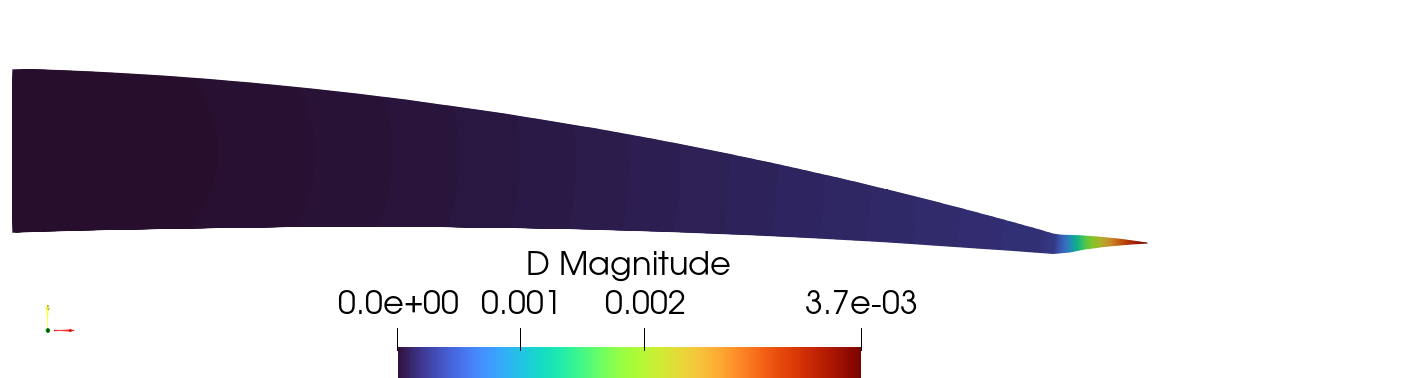
\includegraphics[width=0.45\columnwidth]{Figures/DMAgnitude25GPaCoupling.png}
\caption{Velocity colored flowfield streamlines (right) displacement contours (left) $\Rey=10^5$ and $\mathcal{E}=2.5$ GPa}
\label{fig:25GPA}
\end{figure}
Another goal of deformation control is to keep maximum wing deformation to a minimum in order to avoid damage from large stresses which is critical for control in aeroelastic applications, as it reduces material fatigue caused by vibrations and structural failures caused by high stresses.
%
The equivalent stress contour over the $\mathcal{L}$ segment and its distribution in chordwise direction are presented in Figs.~\ref{fig:stress} and \ref{fig:stress2.5GPa}, respectively.
%
The features learned from the distribution of equivalent stress over the $\mathcal{L}$ segment for $\mathcal{E}=2.5$ GPa shows promising stress relaxation with Young modulus .
%
\begin{figure}[ht!]
\centering
\begin{subfigure}{.4\textwidth}
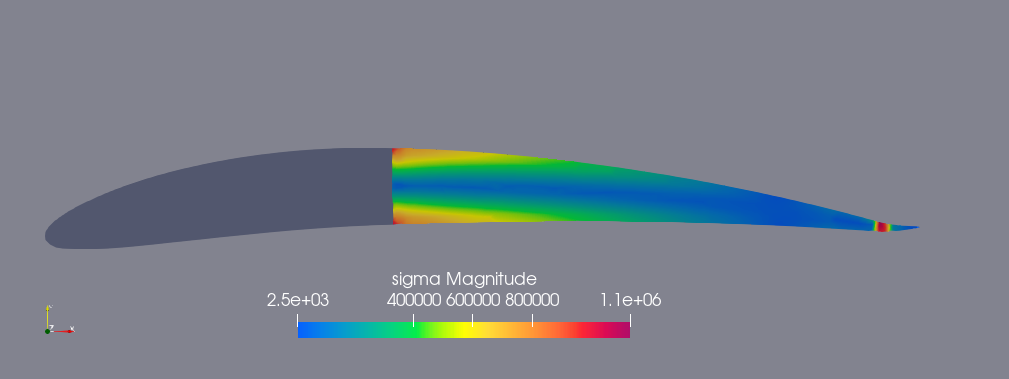
\includegraphics[width=0.99\columnwidth]{Figures/sigma.png}
\caption{\label{fig:stress} Equivalent stress contour over the flexible segment}
\end{subfigure}\\
\begin{subfigure}{.4\textwidth}
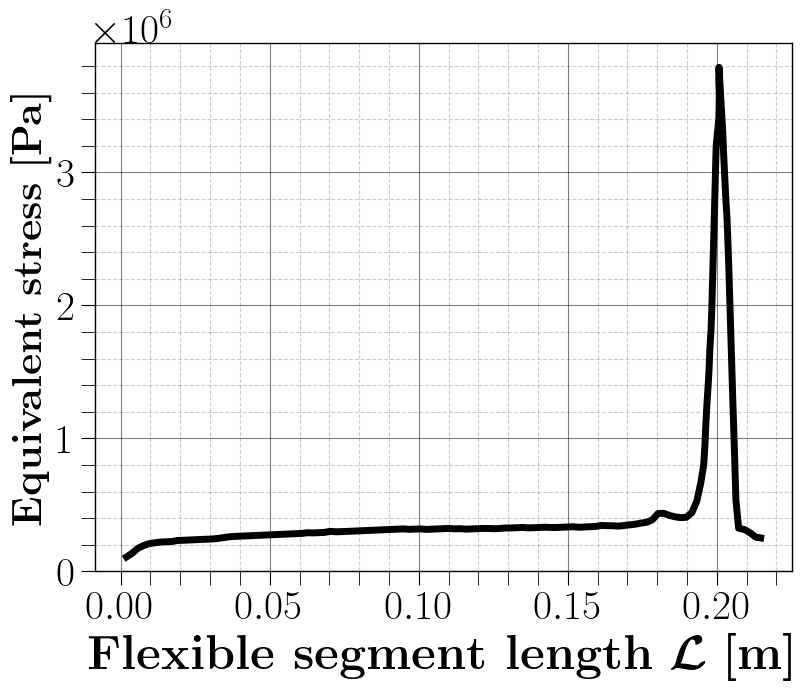
\includegraphics[width=0.99\columnwidth]{figs/equivalentstress.png}
\caption{Chordwise equivalent stress distribution\label{fig:stress2.5GPa}}
\end{subfigure}
\caption{\label{fig:displ} Stress analysis for $\mathcal{E}= 2.5$ GPa }
\end{figure}
%=============================================================
\section{Conclusion}
%=============================================================
Computational modeling can provide a way to develop predictive relationships between morphological traits and their impact on aerodynamic performance through a series of flexibility conditions will be computed using Fluid-Structure interaction (FSI).
%
In this study, we have investigated the stable FSI for turbulent conditions for bio-inspired structure requirements necessary to capture both flow field and structural analysis.
%
One of the primary objectives of evaluations is to investigate the dynamic interaction between low Reynolds number aerodynamic flow and Flexible-Biomimetic NACA6409 as earlier recommended by \citet{gamble2020load}.
%
At an angle of attack $15^{\circ}$, results of the FSI implementation are illustrated for both Young's modulus $\mathcal{E}$ of 689.5 MPa and 2.5 GPa.
%
The study highlights the importance of understanding the stable mechanical properties sufficient for biomimetic adaptive structures and materials.
%
The results suggest that $\mathcal{E}=2.5$ GPa is a promising alternative to replicate the feather and will be used in further investigation of the bird-like wings. 
%=============================================================
\section*{Acknowledgments}
%=============================================================
This work is supported by the International University of Rabat (UIR). Many thanks to the LERMA laboratory for providing the In-house computing resources.
%
The authors would like to thank Imad Kissami and Simlab team for the support with the computing facilities of HPC Simlab-cluster of Mohammed VI Polytechnic University at Benguerir (UM6P).

\bibliography{references.bib}

\end{document}
